\documentclass[10pt,a4paper]{article}
\usepackage[margin=1.8cm]{geometry}
\usepackage[T1]{fontenc}
\usepackage{lmodern}
\usepackage{microtype}
\usepackage{graphicx}
\usepackage{booktabs}
\usepackage{tabularx}
\usepackage{array}
\usepackage{xcolor}
\usepackage{enumitem}
\usepackage[font=small,labelfont=bf]{caption}
\usepackage{tikz}
\usetikzlibrary{positioning,fit,arrows.meta,backgrounds,calc}
\usepackage[colorlinks=true,linkcolor=blue!50!black,urlcolor=blue!50!black]{hyperref}
\setlist{nosep,leftmargin=1.2em}
\setlength{\parskip}{3pt}
\setlength{\parindent}{0pt}
\newcolumntype{L}[1]{>{\raggedright\arraybackslash}p{#1}}
\renewcommand{\arraystretch}{1.12}

\begin{document}

\begin{titlepage}
\centering
\vspace*{0.5cm}
{\Large\bfseries\color[HTML]{7A3B0C} Department of Software Engineering\par}
\vspace{2pt}
{\Large\bfseries NED University of Engineering \& Technology\par}
\vspace{0.6cm}
\IfFileExists{images/ned-logo.png}{
\includegraphics[trim=0 0 138 0,clip,height=3.2cm]{images/ned-logo.png}\par}{}
\vspace{0.4cm}
\rule{0.85\textwidth}{0.6pt}\par
\vspace{0.9cm}
{\Large\bfseries COMPLEX ENGINEERING ACTIVITY (CEA)\par}
\vspace{0.5cm}
{\LARGE\bfseries Design, Deployment and Cloud-Native Enhancement of a Three-Tier Web Application on AWS\par}
\vspace{1.0cm}
\rule{0.85\textwidth}{0.6pt}\par
\vspace{1.0cm}
\begin{minipage}{0.8\textwidth}
\raggedright
\textbf{Course Code \& Title:}\\[3pt]
\hspace*{1.5em}Cloud Computing (SE-490)\\[14pt]
\textbf{Submitted by:}\\[3pt]
\hspace*{1.5em}\begin{tabular}{@{}p{6cm}l@{}}
Nabeed Ali & SE-23054\\
Talha Hussain & SE-23062
\end{tabular}\\[14pt]
\textbf{Submitted to:}\\[3pt]
\hspace*{1.5em}Miss Amna\\[14pt]
\textbf{Source code:}\\[3pt]
\hspace*{1.5em}\url{https://github.com/nabeedjamshedali/Axon}\\[14pt]
\textbf{Platform:}\\[3pt]
\hspace*{1.5em}Amazon Web Services (ap-south-1, Mumbai) $\cdot$ Terraform $\cdot$ Docker $\cdot$ GitHub Actions
\end{minipage}
\vfill
{\large\today}
\end{titlepage}

\section{Introduction and choice of cloud provider}
The Axon product-studio website (a Vite single-page front end) was extended into a genuine three-tier system: an
\textbf{Nginx web tier}, a \textbf{Node.js/Express application tier} (newsletter subscription and contact APIs,
health endpoints) and an \textbf{Amazon RDS PostgreSQL database tier}. The whole environment is described as code
with Terraform, packaged as Docker images, and released by a GitHub Actions pipeline. It runs in
\texttt{ap-south-1} (Mumbai).

\textbf{Why AWS.} (i) One platform provides a managed service for every requirement (VPC, ALB, Auto Scaling, RDS,
ECR, Secrets Manager, CloudWatch, S3), so little undifferentiated infrastructure had to be built by hand;
(ii) Terraform's AWS provider is mature, which makes the deployment reproducible and destroyable, a hard
requirement under a limited credit budget (about US\$38 of free-plan credit); (iii) Mumbai is the closest AWS region to Pakistan,
giving the lowest user latency (its prices are marginally above us-east-1, e.g.\ t3.micro US\$0.0112/h);
(iv) GitHub OIDC federation lets the pipeline deploy without any stored AWS keys.

\section{Architecture and design decisions}
Figure~\ref{fig:arch} shows the final design. Traffic enters through a public Application Load Balancer, reaches
the web tier, which serves static assets and reverse-proxies \texttt{/api/} to an \emph{internal} ALB in front of
the application tier; only the application tier can reach the database. Every compute tier is an Auto Scaling
Group (ASG) spread over two Availability Zones.

\begin{figure}[ht]
\centering
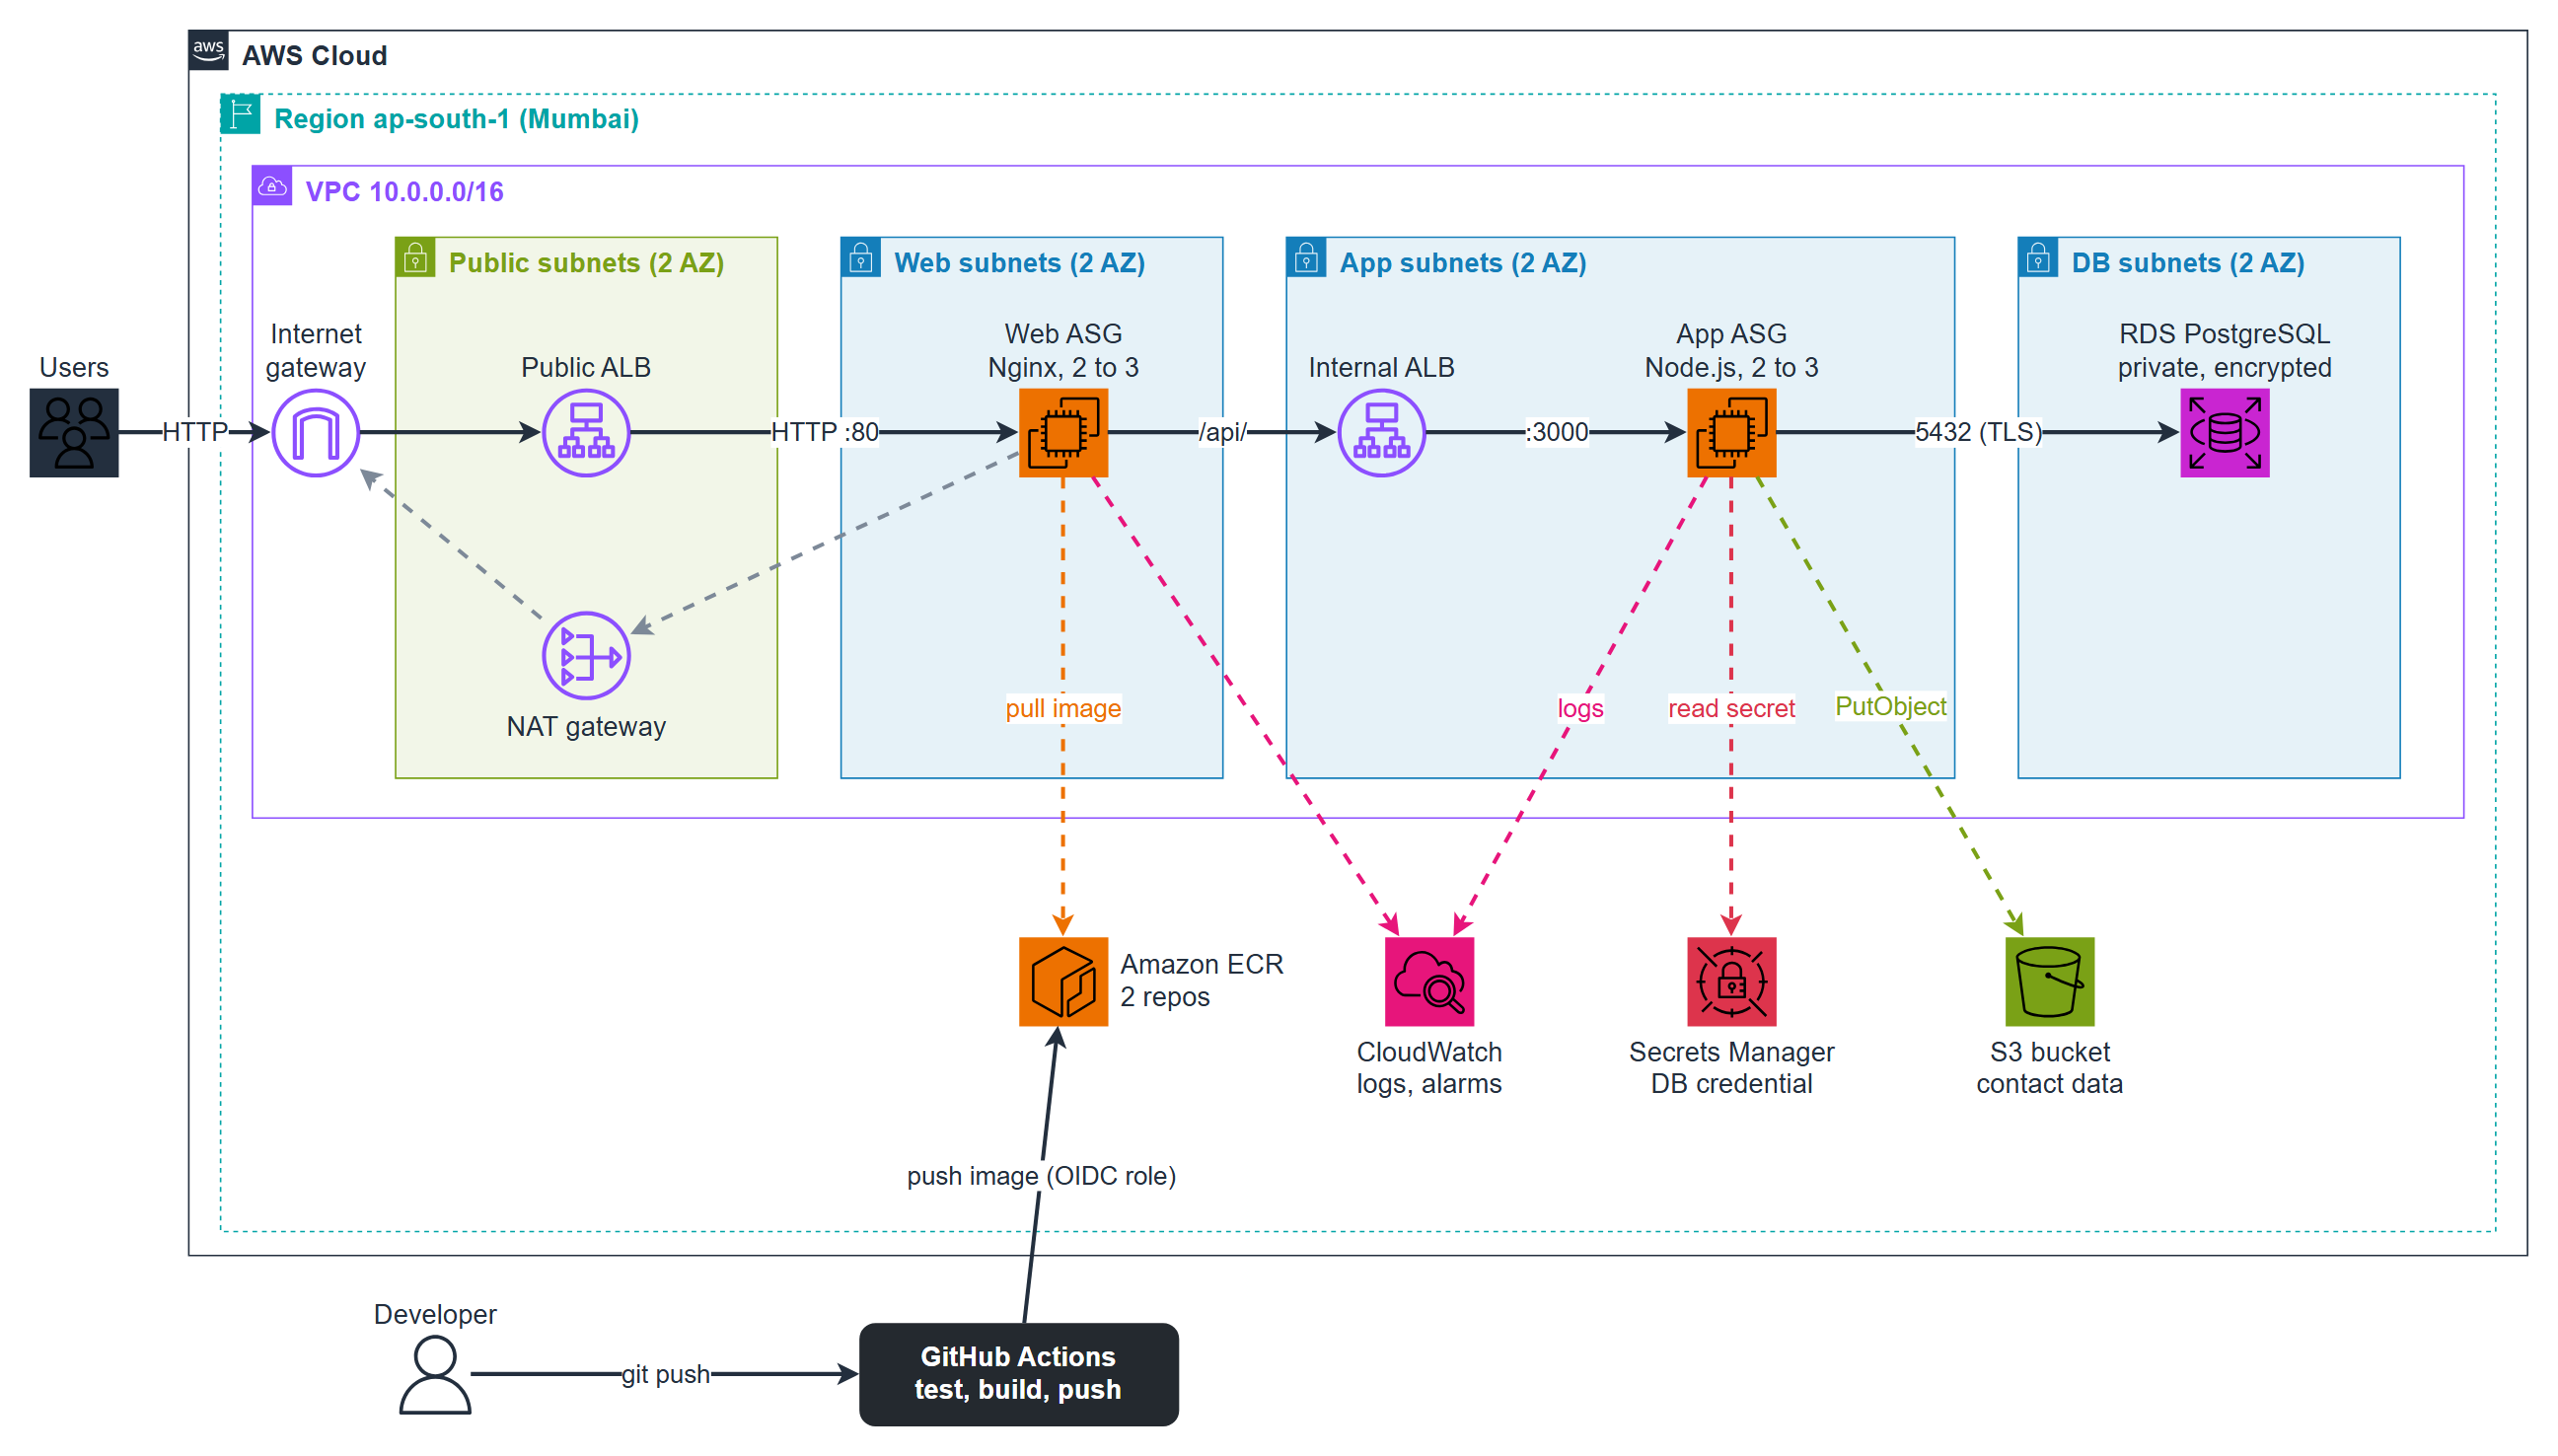
\includegraphics[width=\textwidth]{images/architecture.png}
\caption{Architecture: VPC with two Availability Zones, public ALB, web and application Auto Scaling groups,
internal ALB, private RDS database, managed services and the GitHub Actions CI/CD path (solid = request path,
dashed = management, secret, logging and image-pull paths).}\label{fig:arch}
\end{figure}

\begin{table}[ht]
\centering\small
\begin{tabularx}{\textwidth}{@{}l L{3.7cm} X@{}}
\toprule
\textbf{Tier / layer} & \textbf{AWS service} & \textbf{Role and key decision}\\
\midrule
Network & VPC, 8 subnets, IGW, 1 NAT, route tables, S3 gateway endpoint &
 2 public (ALB, NAT), 2 web, 2 app, 2 DB subnets over two AZs. DB route table has \emph{no} default route. The free S3 endpoint keeps image-layer pulls off the billed NAT.\\
Web & ALB, target group, ASG of t3.micro, Nginx container &
 Serves the built site, adds security headers, proxies \texttt{/api/}, health check \texttt{/healthz}; instances have no public IP.\\
Application & Internal ALB, ASG, Node.js container &
 Stateless business logic; \texttt{/healthz} (liveness, no DB) for the target group, \texttt{/api/health} (DB check) as evidence endpoint.\\
Database & RDS PostgreSQL 16 &
 Managed, encrypted, private; credentials generated and stored by RDS in Secrets Manager.\\
Registry & Amazon ECR (2 repos) & Scan on push, lifecycle rule (keep 10), tags \texttt{:<git-sha>} and \texttt{:latest}.\\
Extras (item 9) & S3, CloudWatch, Terraform, cost estimate &
 S3 stores contact submissions; CloudWatch holds container logs (awslogs driver), 4 alarms and a dashboard; all 84 resources are Terraform-managed.\\
\bottomrule
\end{tabularx}
\caption{Services used and their role in each tier.}
\end{table}

\section{Containerization and CI/CD pipeline}
\textbf{Dockerfiles.} The web image is a multi-stage build (Node builds the Vite bundle; \texttt{nginx:alpine} serves it
and renders its config from a template with \texttt{envsubst}, so the same image works locally and on AWS).
The API image is multi-stage, installs production dependencies only, runs as the unprivileged \texttt{node} user and
declares a \texttt{HEALTHCHECK}. \texttt{docker-compose.yml} runs web, API and PostgreSQL locally on two networks so that
the web container cannot reach the database.

\textbf{Pipeline} (\texttt{.github/workflows/deploy.yml}). On every push to \texttt{main}: (1) \emph{test} job runs the
90 site tests, the production build and the 10 API tests; (2) the \emph{deploy} job assumes an AWS role through
\textbf{GitHub OIDC} (short-lived token, no stored keys), logs in to ECR, builds both images, pushes
\texttt{:<sha>} and \texttt{:latest}, then calls \texttt{StartInstanceRefresh} on both ASGs (rolling, 50\% minimum healthy,
120\,s warm-up), waits for completion and finally smoke-tests the public URL. A \texttt{concurrency} group prevents two
overlapping deployments. Instances pull \texttt{:latest} at boot, so scale-out events also receive the newest release.

\section{Security considerations}
\begin{itemize}
\item \textbf{Segmentation and least privilege.} One security group per tier, each accepting traffic only from the tier in front:
Internet$\to$ALB(80)$\to$web$\to$internal ALB(80)$\to$app(3000)$\to$RDS(5432). Egress is restricted too (e.g.\ the app tier may only reach 5432 in the DB SG and 443 outbound). No security group allows SSH; administration uses SSM Session Manager.
\item \textbf{Secrets.} RDS generates the master password and keeps it in Secrets Manager. The app instance role may read \emph{only that secret}; the boot script writes it to a root-only (0600) env file used by the container. Nothing sensitive is in Git, images, user-data or CI. The pipeline needs no AWS secret at all because of OIDC; the trust policy accepts only the \texttt{main} branch of this repository (pinned by immutable repository ID).
\item \textbf{IAM.} Separate web/app instance roles (ECR pull for their own repository, write to their own log group; the app additionally \texttt{s3:PutObject} on \texttt{contacts/*}). The CI role can push to the two ECR repos and refresh the two ASGs, nothing else.
\item \textbf{Data and host hardening.} EBS, RDS and S3 encryption at rest; S3 public access fully blocked; IMDSv2 required; database not publicly accessible and in subnets with no internet route; ECR scan-on-push; Nginx security headers; non-root container.
\end{itemize}

\section{Testing results}
\begin{table}[ht]
\centering\small
\begin{tabularx}{\textwidth}{@{}L{4.2cm} X@{}}
\toprule
\textbf{Test} & \textbf{Result}\\
\midrule
Unit/integration (local) & API: 10/10 pass (validation, idempotent subscribe, DB-failure handling); site: 90/90 pass.\\
Local three-tier run & \texttt{docker compose up}: site 200, \texttt{/api/health} DB up, duplicate subscription handled, row visible in PostgreSQL.\\
Infrastructure as code & \texttt{terraform validate} OK; plan 84 resources; apply succeeded; follow-up plan showed no drift.\\
Automated deployment & Run \#1 failed at the OIDC step (diagnosed from CloudTrail: GitHub now issues subject claims containing immutable IDs; trust policy updated). Run \#2: all jobs green in 11\,m\,44\,s (tests 11\,s; build, push, rolling deploy and smoke test 11\,m\,26\,s). The footer of the live site now reports the new commit (\texttt{v6b6a2db}).\\
Load balancing & Six consecutive calls to \texttt{/api/health} through the public ALB alternated between two app instances in \texttt{ap-south-1a} and \texttt{ap-south-1b}.\\
Write path & POST \texttt{/api/subscribe} through ALB $\to$ Nginx $\to$ internal ALB $\to$ API $\to$ RDS returned 201.\\
Failure injection & One app instance was terminated while sending a request every 2\,s for 120\,s: 56/60 requests succeeded; the 4 failures (HTTP 502/time-out) all occurred in the first 16\,s, before ALB health checks removed the dead target. The ASG had a replacement \texttt{InService} and healthy at the end of the window.\\
\bottomrule
\end{tabularx}
\caption{Test results. Console screenshots for all components are in the separate evidence document.}
\end{table}

\begin{figure}[ht]
\centering
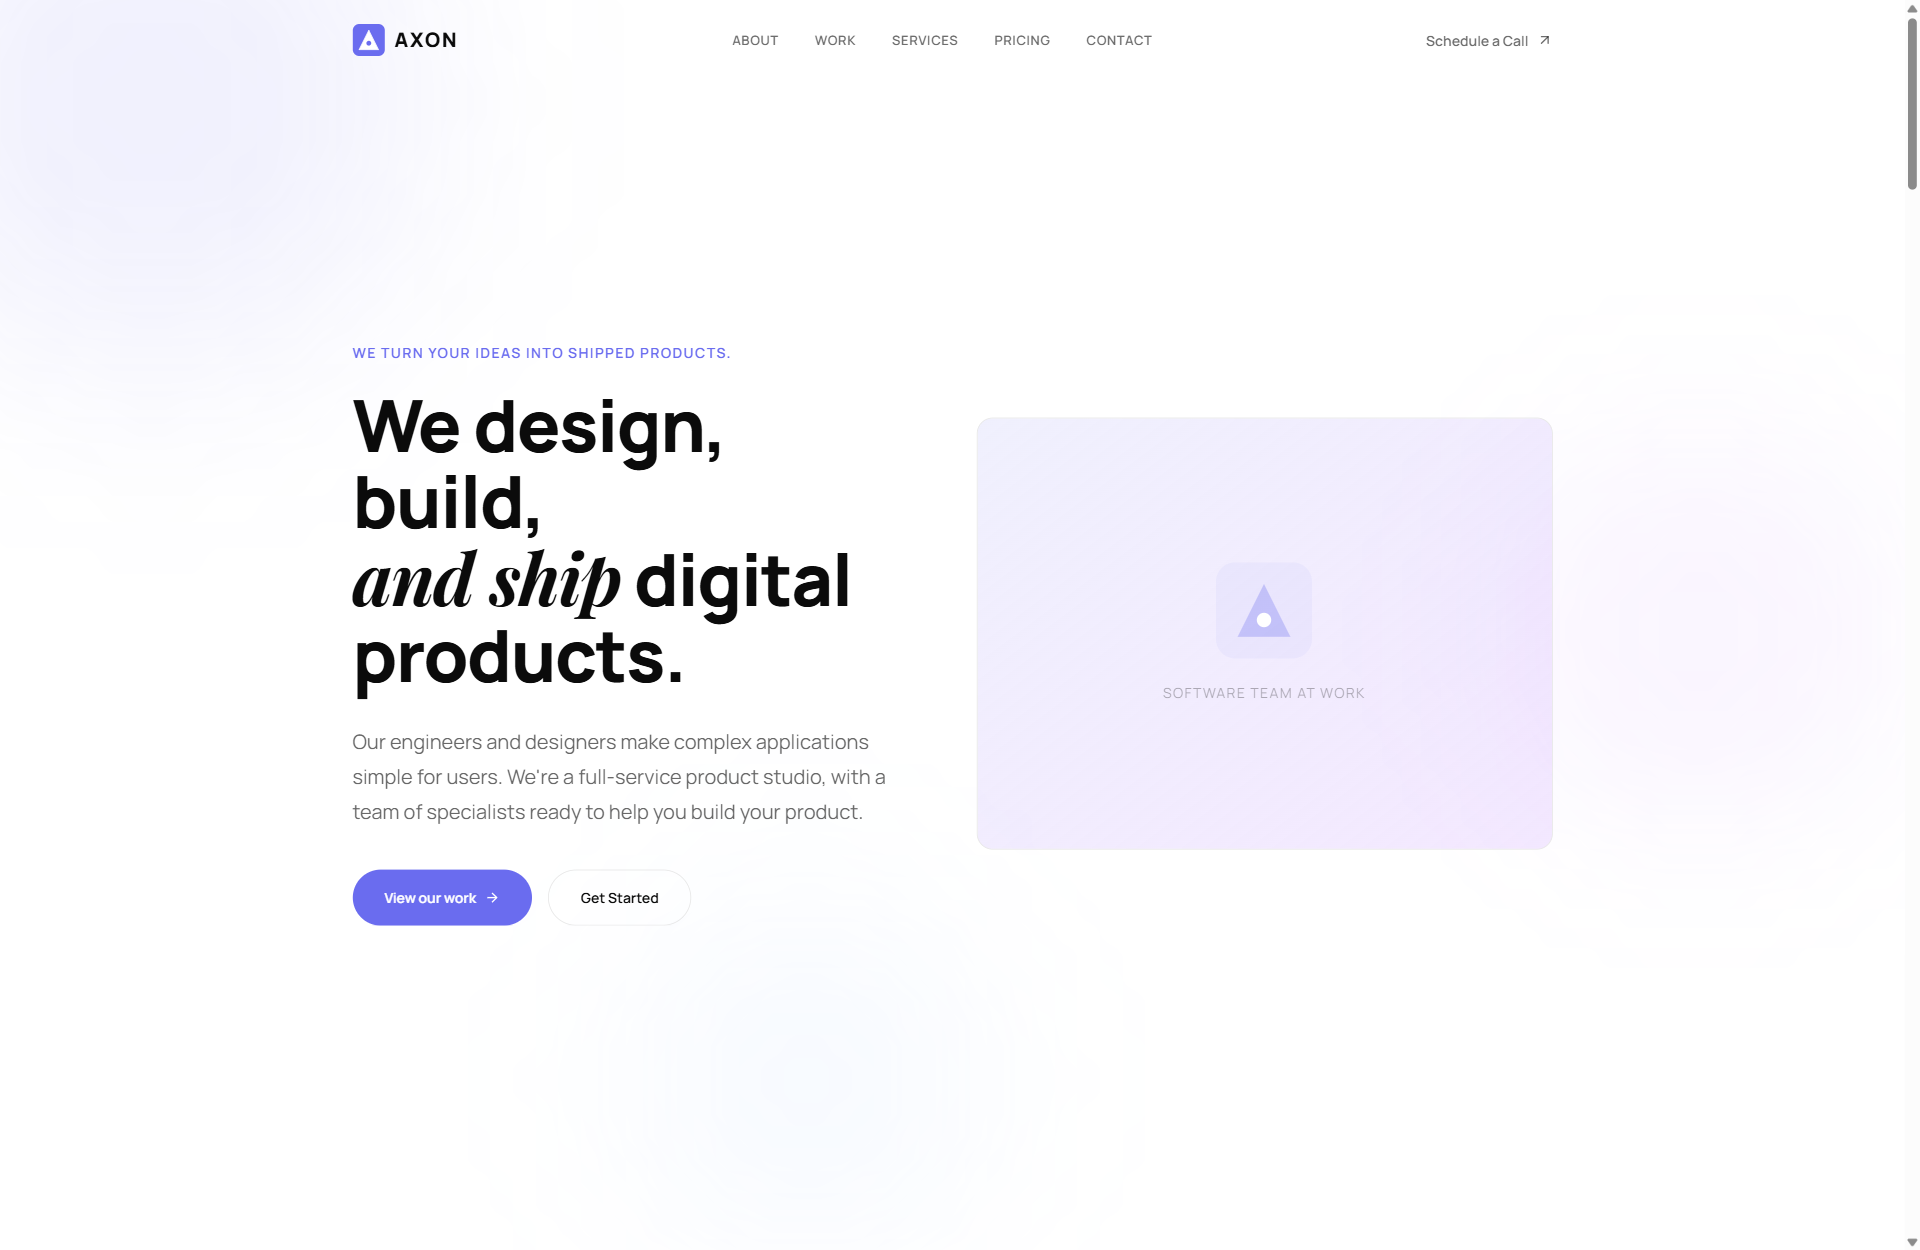
\includegraphics[width=0.48\textwidth]{images/21-app-home.png}\hfill
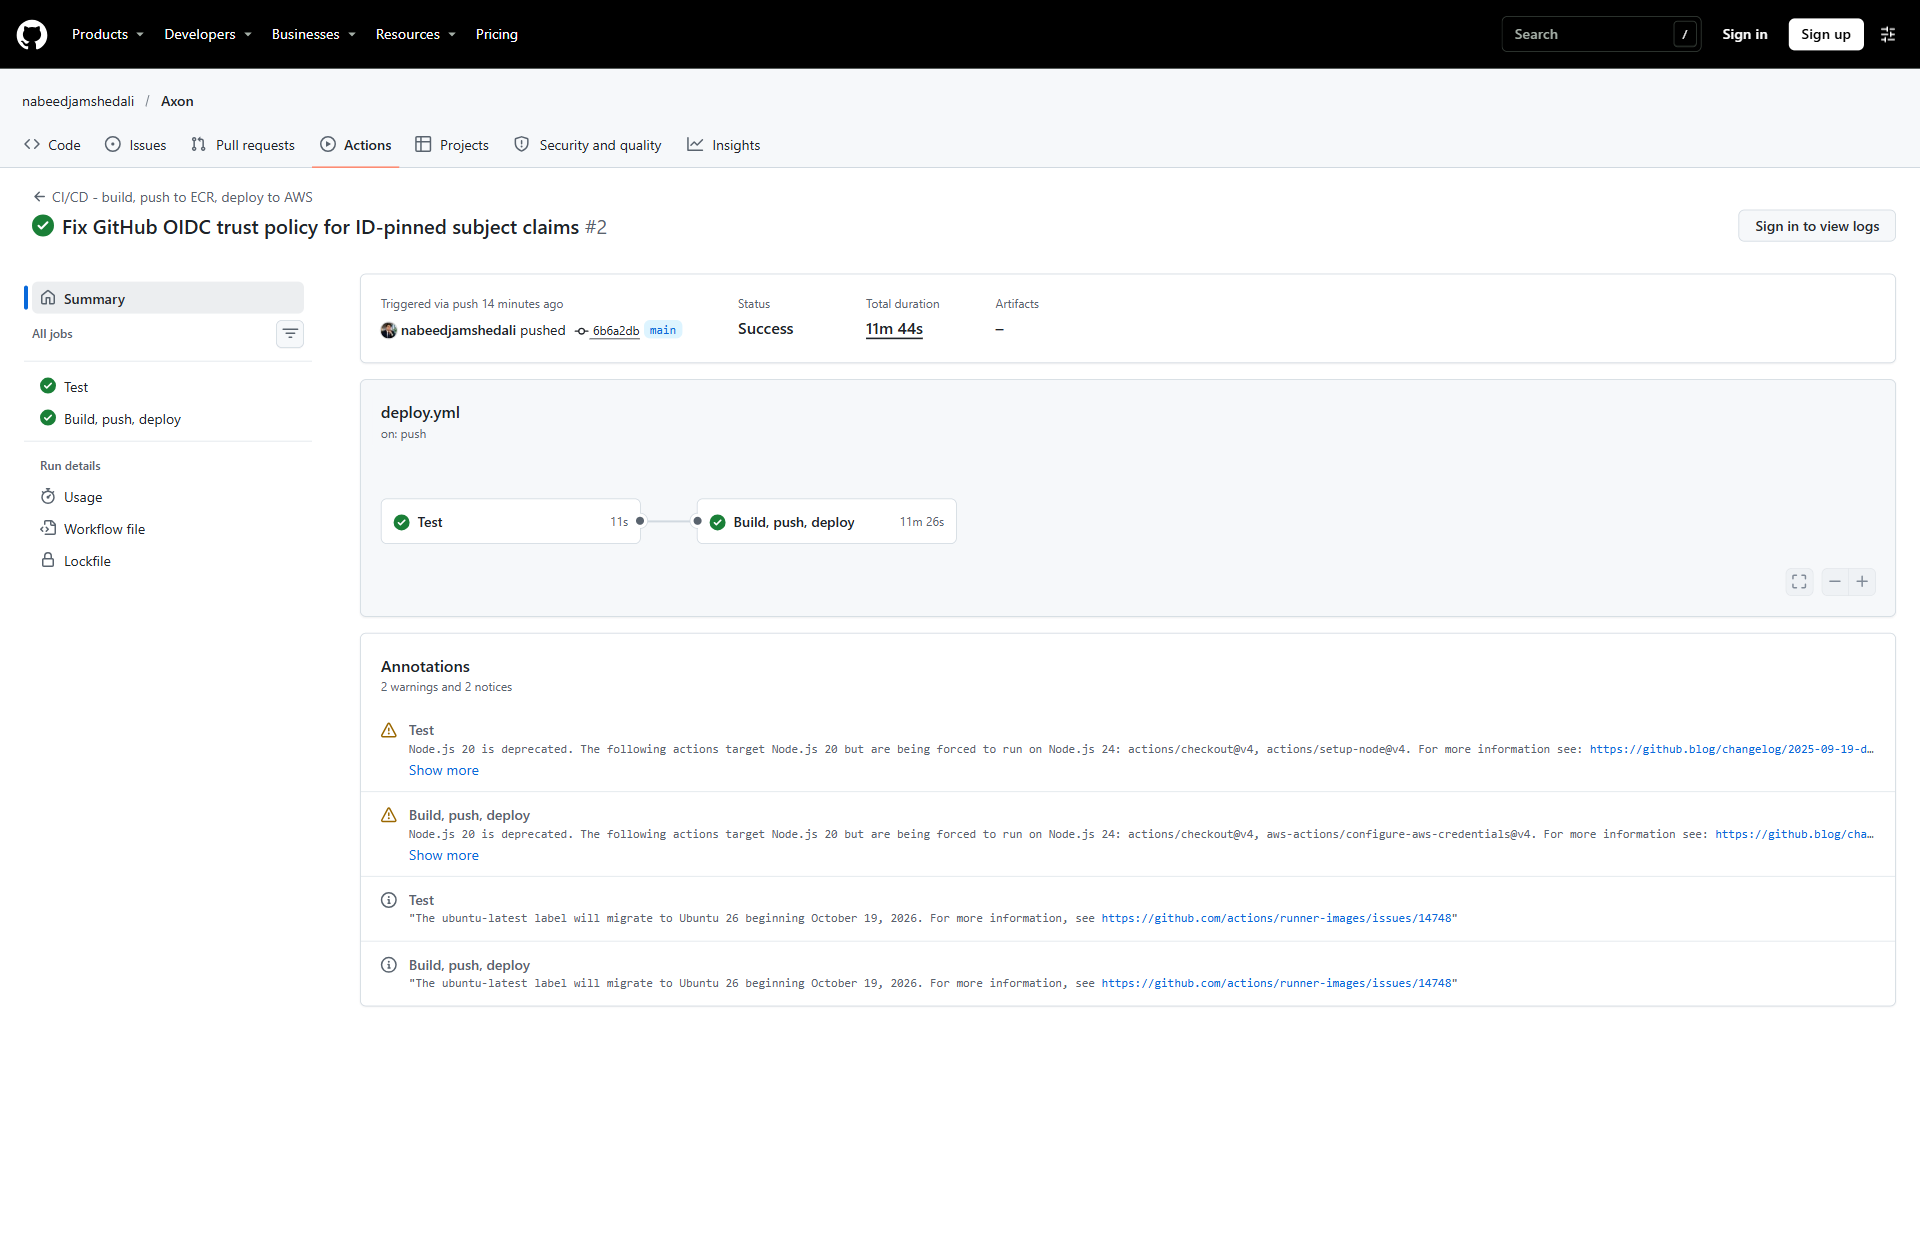
\includegraphics[width=0.48\textwidth]{images/23-github-actions-run.png}
\caption{Left: the running application reached through the ALB. Right: the successful GitHub Actions run.}
\end{figure}

\section{Non-functional requirements (NFR) justification}
\begin{table}[ht]
\centering\footnotesize
\begin{tabularx}{\textwidth}{@{}L{2.0cm} X X@{}}
\toprule
\textbf{NFR} & \textbf{Design / implementation decision} & \textbf{Known limitation $\to$ improvement}\\
\midrule
Scalability & Stateless containers (state only in RDS/S3); ALB spreads load; ASGs scale 2$\to$3 on CPU target tracking; scale-out instances boot from \texttt{:latest}. & Database is a single instance: add read replicas / RDS Proxy; scale on request count as well as CPU.\\
Availability / reliability & Two AZs for every tier, two ALBs, $\geq$2 instances per tier, ELB-based health checks with automatic replacement; measured recovery in the failure test. & RDS is \emph{single-AZ} (cost); single NAT is an AZ-level SPOF for egress only. $\to$ \texttt{db\_multi\_az=true}; one NAT per AZ.\\
Elasticity & Target-tracking policies add/remove instances automatically (min 2, max 3); the whole stack can be destroyed and recreated by Terraform. & Small max size and CPU-only trigger; $\to$ larger bounds and scheduled scaling.\\
Security & Section~4: per-tier SGs, private subnets, least-privilege IAM, managed secret, OIDC pipeline, encryption, no SSH. & Traffic is HTTP (no domain/ACM certificate); app uses the DB master user. $\to$ HTTPS listener + WAF; dedicated least-privilege DB role; TLS CA pinning.\\
Maintainability / deployability & Everything in Git: Dockerfiles, Terraform, workflow; one push triggers test, build, push and rolling deploy with no manual step or SSH; \texttt{:<sha>} tags allow rollback. & Rollback is manual (re-tag). $\to$ automatic rollback on failed smoke test; blue/green.\\
Performance / latency & Mumbai region (closest to users in Pakistan); Nginx gzip and long-lived cache headers for hashed assets; ALBs in the same region/AZs; S3 endpoint avoids NAT hairpin. & No CDN or cache layer, t3.micro burstable CPU. $\to$ CloudFront in front of the ALB, ElastiCache, larger instances.\\
Cost efficiency & One shared NAT, t3.micro/db.t3.micro, 8\,GB gp3 volumes, 7-day log retention, ECR lifecycle policy, free S3 endpoint, budget alerts at US\$15/30, and destruction of the stack after evidence capture (Section~7). & Idle cost is still dominated by NAT and ALBs. $\to$ consolidate ALBs, Savings Plans, Graviton.\\
Portability & Docker images contain all runtime dependencies; configuration via environment variables; the same images run unchanged under docker-compose, on EC2 and could run on EKS/ECS or another cloud. & Terraform code, ALB/ASG/RDS specifics and OIDC trust are AWS-specific. $\to$ keep an abstraction layer or add Kubernetes manifests.\\
\bottomrule
\end{tabularx}
\caption{Mapping of design decisions to NFRs, with honest limitations.}
\end{table}

\section{Cost estimate and optimization}
Monthly cost of the full environment at 730\,h, using AWS Price List rates for \texttt{ap-south-1}
(t3.micro US\$0.0112/h, NAT US\$0.056/h plus US\$0.056/GB, ALB US\$0.0239/h plus LCU, db.t3.micro US\$0.026/h,
public IPv4 US\$0.005/h; storage and small items approximate):

\begin{table}[ht]
\centering\small
\begin{tabular}{@{}lr@{\qquad}lr@{}}
\toprule
4 $\times$ EC2 t3.micro & 32.70 & 2 $\times$ public IPv4 on ALB + 1 on NAT & 10.95\\
1 $\times$ NAT gateway (+10\,GB) & 41.44 & EBS 32\,GB gp3 (approx.) & 2.92\\
2 $\times$ ALB (+LCU, approx.) & 36.29 & S3, CloudWatch, Secrets, ECR (approx.) & 1.90\\
RDS db.t3.micro + 20\,GB (approx.) & 21.60 & \textbf{Total per month} & \textbf{$\approx$ 147.8}\\
\bottomrule
\end{tabular}
\caption{Estimated monthly cost (US\$), about US\$0.20 per hour or US\$4.9 per day.}
\end{table}
\textbf{Optimizations.} (1) \emph{Implemented:} a single shared NAT gateway instead of one per AZ saves US\$40.9/month (28\%),
and the S3 gateway endpoint keeps ECR layer traffic off the metered NAT. (2) \emph{Implemented:} the environment is ephemeral:
Terraform brings it up for the evaluation and \texttt{terraform destroy} removes it, so the actual spend for a few days of testing
is roughly US\$5/day rather than US\$148/month. (3) \emph{Proposed:} merge the internal ALB into the public one with path-based
routing (saves about US\$18/month), and (4) move to Graviton \texttt{t4g.micro} instances (about 20\% cheaper compute).

\section{Conclusion and known limitations}
All mandatory requirements were met with an automated, reproducible, secured three-tier deployment: network layer, containerized web and
application tiers, managed database, container registry, CI/CD, load balancing with auto scaling, per-tier security and secret management, plus
four cloud-native enhancements (S3, CloudWatch, Terraform, cost analysis). Honest gaps: no HTTPS, single-AZ database, single NAT, CPU-only scaling,
local Terraform state (an S3 backend with locking is recommended for teams), and Kubernetes was not used. Each has a concrete improvement path in Section~6.

\end{document}
